% !TeX program = xelatex
%% 부득이하게 pdflatex을 사용해야 할 경우 위의 magic comment를 제거하십시오.

%%%%%%%%%%%%%%%%%%%%%%%%%%%%%%%%%%%%%%%%%
% The Legrand Orange Book
% LaTeX Template
% Version 2.2 (30/3/17)
%
% This template has been downloaded from:
% http://www.LaTeXTemplates.com
%
% Original author:
% Mathias Legrand (legrand.mathias@gmail.com) with modifications by:
% Vel (vel@latextemplates.com)
%
% License:
% CC BY-NC-SA 3.0 (http://creativecommons.org/licenses/by-nc-sa/3.0/)
%
% Compiling this template:
% This template uses biber for its bibliography and makeindex for its index.
% When you first open the template, compile it from the command line with the 
% commands below to make sure your LaTeX distribution is configured correctly:
%
% 1) pdflatex main
% 2) makeindex main.idx -s StyleInd.ist
% 3) biber main
% 4) pdflatex main x 2
%
% After this, when you wish to update the bibliography/index use the appropriate
% command above and make sure to compile with pdflatex several times 
% afterwards to propagate your changes to the document.
%
% This template also uses a number of packages which may need to be
% updated to the newest versions for the template to compile. It is strongly
% recommended you update your LaTeX distribution if you have any
% compilation errors.
%
% Important note:
% Chapter heading images should have a 2:1 width:height ratio,
% e.g. 920px width and 460px height.
%
%%%%%%%%%%%%%%%%%%%%%%%%%%%%%%%%%%%%%%%%%

\documentclass{gshs_thesis}

\graphicspath{{images/}}
% 이곳에 필요한 별도의 패키지들을 적어넣으시오.
%\usepackage{...}
\usepackage{verbatim} % for commment, verbatim environment
\usepackage{spverbatim} % automatic linebreak verbatim environment
\usepackage{listings}
\lstset{
	basicstyle=\small\ttfamily,
	columns=flexible,
	breaklines=true
}
\usepackage{hologo}

% -----------------------------------------------------------------------
%                   이 부분은 수정하지 마시오.
% -----------------------------------------------------------------------
\titleheader{졸업논문청구논문}
\school{과학영재학교 경기과학고등학교}
\approval{위 논문은 과학영재학교 경기과학고등학교 졸업논문으로\\
졸업논문심사위원회에서 심사 통과하였음.}
\chairperson{심사위원장}
\examiner{심사위원}
\apprvsign{(인)}
\korabstract{초 록}
\koracknowledgement{감사의 글}
\korresearches{연 구 활 동}

%: ----------------------------------------------------------------------
%:                  논문 제목과 저자 이름을 입력하시오
% ----------------------------------------------------------------------
\title{한글 제목} %한글 제목
\engtitle{English Title} %영문 제목
\korname{홍 길 동} %저자 이름을 한글로 입력하시오 (글자 사이 띄어쓰기)
\engname{Hong, Gil-Dong} %저자 이름을 영어로 입력하시오 (family name, personal name)
\chnname{洪 吉 東} %저자 이름을 한자로 입력하시오 (글자 사이 띄어쓰기)
\studid{14201} %학번을 입력하시오

%------------------------------------------------------------------------
%                  심사위원과 논문 승인 날짜를 입력하시오
%------------------------------------------------------------------------
\advisor{Mok, Chinook}  %지도교사 영문 이름 (family name, personal name)
\judgeone{박 승 원} %심사위원장
\judgetwo{이 주 찬}   %심사위원1
\judgethree{목 진 욱} %심사위원2(지도교사)
\degreeyear{2017}   %졸업 년도
\degreedate{2016}{11}{13} %논문 승인 날짜 양식

%------------------------------------------------------------------------
%                  논문제출 전 체크리스트를 확인하시오
%------------------------------------------------------------------------
\checklisttitle{[논문제출 전 체크리스트]} %수정하지 마시오
\checklistI{1. 이 논문은 내가 직접 연구하고 작성한 것이다.} %수정하지 마시오
% 이 항목이 사실이라면 다음 줄 앞에 "%"기호 삽입, 다다음 줄 앞의 "%"기호 제거하시오
\checklistmarkI{$\square$}
%\checklistmarkI{$\text{\rlap{$\checkmark$}}\square$}
\checklistII{2. 인용한 모든 자료(책, 논문, 인터넷자료 등)의 인용표시를 바르게 하였다.} %수정하지 마시오
% 이 항목이 사실이라면 다음 줄 앞에 "%"기호 삽입, 다다음 줄 앞의 "%"기호 제거하시오
\checklistmarkII{$\square$}
%\checklistmarkII{$\text{\rlap{$\checkmark$}}\square$}
\checklistIII{3. 인용한 자료의 표현이나 내용을 왜곡하지 않았다.} %수정하지마시오
% 이 항목이 사실이라면 다음 줄 앞에 "%"기호 삽입, 다다음 줄 앞의 "%"기호 제거하시오
\checklistmarkIII{$\square$}
%\checklistmarkIII{$\text{\rlap{$\checkmark$}}\square$}
\checklistIV{4. 정확한 출처제시 없이 다른 사람의 글이나 아이디어를 가져오지 않았다.} %수정하지 마시오
% 이 항목이 사실이라면 다음 줄 앞에 "%"기호 삽입, 다다음 줄 앞의 "%"기호 제거하시오
\checklistmarkIV{$\square$}
%\checklistmarkIV{$\text{\rlap{$\checkmark$}}\square$}
\checklistV{5. 논문 작성 중 도표나 데이터를 조작(위조 혹은 변조)하지 않았다.} %수정하지 마시오
% 이 항목이 사실이라면 다음 줄 앞에 "%"기호 삽입, 다다음 줄 앞의 "%"기호 제거하시오
\checklistmarkV{$\square$}
%\checklistmarkV{$\text{\rlap{$\checkmark$}}\square$}
\checklistVI{6. 다른 친구와 같은 내용의 논문을 제출하지 않았다.} %수정하지 마시오
% 이 항목이 사실이라면 다음 줄 앞에 "%"기호 삽입, 다다음 줄 앞의 "%"기호 제거하시오
\checklistmarkVI{$\square$}
%\checklistmarkVI{$\text{\rlap{$\checkmark$}}\square$} % usepackage 등의 명령어는 여기에.
\usepackage{cite}
\usepackage{textcomp}
\usepackage{tocloft}
\setlength{\cftbeforesecskip}{0pt}
\setlength{\cftbeforesubsecskip}{0pt}
\setlength{\cftbeforesubsubsecskip}{0pt}

%----------------------------------------------------------------------------------------
%	PACKAGES AND OTHER DOCUMENT CONFIGURATIONS
%----------------------------------------------------------------------------------------
%\documentclass[11pt,fleqn]{book_main} % Default font size and left-justified equations
%\documentclass[11pt,fleqn]{book} % Default font size and left-justified equations
%----------------------------------------------------------------------------------------


%----------------------------------------------------------------------------------------
%	TITLE PAGE
%----------------------------------------------------------------------------------------
\def\subject{관측 천문학} % subject
%\def\unittitle{python 기초} % Title
\title{python 기초} % Title
\author{Kiehyun \textsc{Park} (guitar79@naver.com) % Author name
\def\school{Gyeonggi Science High School for the Gifted}
% command to print the title page with above variables
\date{\today}



\begin{document}
	%
%----------------------------------------------------------------------------------------
%	TITLE PAGE
%----------------------------------------------------------------------------------------


%%%%%%%%%%%%%%%%%%%%%%%%%%%%%%
%%%define title page layout%%%
%%%%%%%%%%%%%%%%%%%%%%%%%%%%%%
\renewcommand{\maketitle}{%
	\thispagestyle{empty}   %%%% 제 1 타이틀 페이지
	\begin{center}
		\begin{minipage}[h][20mm][c]{\textwidth}
			{\large\bfseries \subject  \\
		\end{minipage}
		\vspace{80mm}
		\begin{minipage}[h][50mm][c]{\textwidth}
			\begin{center}
				\huge\bfseries \title  \\
			\end{center}
		\end{minipage}
		\vspace{20mm}
		\begin{minipage}[h][15mm][c]{\textwidth}
			\begin{center}
				\normalsize\bfseries \date
			\end{center}
		\end{minipage}
		%		\vspace{20mm}
		\begin{minipage}[h][15mm][c]{\textwidth}
			\begin{center}
				\normalsize\bfseries \author \\
				(\email)
			\end{center}
		\end{minipage}
		\begin{minipage}[h][15mm][c]{\textwidth}
		\begin{center}
			\large\bfseries \school \\
		\end{center}
	\end{minipage}

	\end{center}
}

%  \null\vfill
 % Title page
	\maketitle
	\renewcommand{\thepage}{\arabic{page}}
	\setcounter{page}{1}
	\section{Python}

\subsection{Python 소개}\index{Python 소개}

파이썬(Python)은 1991년 프로그래머인 귀도 반 로섬(Guido van Rossum)이 발표한 고급 프로그래밍 언어로, 플랫폼 독립적이며 인터프리터식, 객체지향적, 동적 타이핑(dynamically typed) 대화형 언어이다. 파이썬이라는 이름은 귀도가 좋아하는 코미디 〈Monty Python's Flying Circus〉에서 따온 것이다.

파이썬은 비영리의 파이썬 소프트웨어 재단이 관리하는 개방형, 공동체 기반 개발 모델을 가지고 있다. C언어로 구현된 C파이썬 구현이 사실상의 표준이다.

파이썬은 무료이며 누구나 다운받아 사용 가능 하다.


\subsection{Python 설치}\index{Python 설치}

파이썬은 무료이며 누구나 다운받아 사용 가능 하다.


\subsection{Python 시작하기}\index{}

The Python programming language is a very popular, versatile, and (with its many extensions) very powerful tool. An interpreter that runs scripts in the programming language Python is freely distributed, and it may already be installed on your computer. There are many excellent free on-line tutorials on Python, including https://docs.python.org/ and Coursera classes beginning with https://www.coursera.org/learn/python. This class assumes that you have access to a tutorial or documentation, and will demonstrate how you can use the powers of Python to simulate things that happen in the natural world. The only way to learn a programming language is by doing something with it; just reading about it, it doesn't sink in in the same way. This class provides an opportunity for someone new to coding to get started, by providing detailed instructions for building a series of simple models applicable to the climate sciences. I've tried to write the instructions as if they were to go with some kind of kit, like to build a toy sailboat. The instructions are meant to make it as clear and easy as possible to succeed. By doing so, you will learn a lot about climate and Python both!

Using Python for numerical computation requires extensions which you will probably have to install. First is a numerical module called numpy (pronounced num-pie), and second, you'll also need a plotting module called matplotlib. On my Macintosh, I succeeded in using a package called anaconda (https://www.continuum.io/downloads), by installing their minimum package they call miniconda, and using that to install numpy and matplotlib. At the beginnings of your python scripts you will need to start these up using lines

\begin{code}[]
	%	\begin{align}
	\begin{lstlisting}
	
	import numpy
	import matplotlib
	\end{lstlisting}
	%		\end{align}
\end{code}

%where you should replace model_name.py with whatever the name of your script file is.
where you should replace modelname.py with whatever the name of your script file is.

\subsection{Editing Files}\index{Editing Files}

To create and edit Python scripts or Fortran source files, you will need to find or install an editor which can write plain text files. Word processors such as Word or TextEdit may be able to save clean text files, if you specifically look for that. A way to check is to type “more <filename>” in a terminal window, where you substitute the name of the file you want to inspect for <filename>, which will give you a screen-full of the file at a time. If it looks like plain letters of python text, you’re good. Examples of formats which won’t work include files with the suffix .doc, .docx, .rtf, and .pdf.

Alternatively, you may find some integrated programming environment for your computer that shows you the editable python source code in one part of a window, and output in another part.

\subsection{Getting your code to work}\index{Getting your code to work}

Create your first script by copying pieces from some example script. When you first try to run it, it probably will have some syntax errors that will prevent the Python interpreter from working. The interpreter will tell you what line it decided it had to give up, which is usually the line where the error is, but not always. It can be a problem at an earlier line, like a mismatched parenthesis in a line above. Sometimes the only way to find where a problem line is, is to temporarily delete or comment out whole blocks of a code, until it starts running. Google is your friend here; you can copy the entire error message into the Google search box, add the word python or anything else relevant to what you’re trying to do, and probably you will find posts where the same question has been asked and answered. In particular, a web site called stackoverflow.com is a treasure chest of helpful information.

Once the code gets correct enough to run, it will probably give wrong answers that will require debugging. The simplest way to probe the numbers that the code is creating is to put in temporary print statements, printing out values of variables. Another fancier option is to use a debugger, which allows you to stop the code at some line number, step forward a bit at a time, and ask it interactively what all the variable values are, and even change them on the fly.

A general strategy is to find or create the simplest possible script that works correctly, then improve it or add stuff to it in stages. A working spreadsheet will make debugging much easier by providing lots of numbers to compare to. Also, getting the same answers in two formats (spreadsheet and code) gives a lot of reassurance that there aren't random typo-type bugs in either format. Simplify a strangely-behaving code until it gets so simple that it works, then add the complexity back in, one step at a time, until you get that working also. You can use comment marks (\#) to "comment out" lines of code temporarily.

You will be uploading your codes for automatic checking, and also for peer review. The automatic checking needs to have your code set up particular ways, to take some numbers as input, print out other numbers as output, with no extra text or on-screen plotting (matplotlib). The code checker will run your code through some paces and give what we hope will be helpful feedback on your calculations. The peer review will be to assess your coding "style", whether you have useful comments in the code, the variable names make sense, the code is logically structured: things like that. After you submit your code, you will be asked to evaluate the codes of others.




\section{파이썬 라이브러리}\index{파이썬 라이브러리}

지금부터 사용할 아이브러리와 과학계산용 파이썬 환경에 익숙하지 않은 사용자를 위해 간단히 라이브러리를 소개한다.

\subsection{Numpy}\index{Numpy}

NumPy(http://numpy.org)는 Numerical Python의 줄임말로, 과학계산용 파운데이션 패키지이다. 다음은 NumPy의 기능이다.


\begin{itemize}
	\item{빠르고 효율적인 다차원 배열 객체ndarray}
	\item{배열 원소를 다루거나 배열 간의 수학 계산을 수행하는 함수}
	\item{디스크로부터 배열 기반의 데이터를 읽거나 쓸 수 있는 도구}
	\item{선형대수 계산, 푸리에 변환, 난수 발생기}
	\item{파이썬과 C, C++ 그리고 포트란 코드를 통합하는 도구}
\end{itemize}


NumPy는 파이썬에 빠른 배열 처리 기능을 제공하며, 데이터 분석에서는 알고리즘에 사용할 데이터 컨테이너의 역할을 한다. 수이데이터라면 NumPy 배열은 파이선 기본 자료 구조보다 훨씬 효율적인 방법으로 데이터를 저장하고 다룰 수 있다. 또한 C나 포트란 같은 저수준 언어로 이루어진 라이브러리는 NumPy 배열에 저장된 데이터를 복사하지 않고 사용할 수 있다. 


\subsection{Matplotlib}\index{Theorems}

https://matplotlib.org/

matplotlib \은 그래프나 2차원 데어터 시각화를 생성하는 유명한 파이썬 라이브러리다. Jhn D. Hunter \가 만들었고, 지금은 만은 배발 팀이 유지하고 있다. 출판물에 필요한 그래프를 만드는 데 맞춰졌으며 IPython에 통합되어 있어 편리하게 데이터를 살펴보고 그래프를 만들수 있다. IPython에서 matplotlib \로 생성한 그래프는 그래프 창에 있는 툴바로 특정 부분을 확대하거나 그래프의 여기저기를 인터랙트브하게 살펴볼 수 있다.


\subsection{matplotlib basemap toolkit}\index{basemap}

The matplotlib basemap toolkit is a library for plotting 2D data on maps in Python. It is similar in functionality to the matlab mapping toolbox, the IDL mapping facilities, GrADS, or the Generic Mapping Tools. PyNGL and CDAT are other libraries that provide similar capabilities in Python.

Basemap does not do any plotting on it’s own, but provides the facilities to transform coordinates to one of 25 different map projections (using the PROJ.4 C library). Matplotlib is then used to plot contours, images, vectors, lines or points in the transformed coordinates. Shoreline, river and political boundary datasets (from Generic Mapping Tools) are provided, along with methods for plotting them. The GEOS library is used internally to clip the coastline and polticial boundary features to the desired map projection region.

Basemap is geared toward the needs of earth scientists, particularly oceanographers and meteorologists. Jeff Whitaker originally wrote Basemap to help in his research (climate and weather forecasting), since at the time CDAT was the only other tool in python for plotting data on map projections. Over the years, the capabilities of Basemap have evolved as scientists in other disciplines (such as biology, geology and geophysics) requested and contributed new features.


	%\chapterimage{chapter_head_1.pdf} % Chapter heading image
\chapter{기상청 일기 예보}

\section{예보가 나오는 과정}

예보가 나오기까지는 기상실황파악 → 자료수집 → 분석 → 예보작성 → 통보 과정을 거친다. 

\section{기상실황 파악}

\subsection{지상기상 관측}
전국 76개소의 기상관서에서 하늘상태, 시정 등의 목측 (目測 ) 요소를 관측하고 있으며, 기온, 습도, 강수량, 바람, 기압 등은 자동기상관측장비를 이용하여 1분 간격으로 관측되고 있다. 또한, 기상관서가 없는 500여 소에서는 방재용 자동기상관측장비를 이용하여 기온, 풍향, 풍속, 강수량, 강수 유무를 1분 간격으로 관측하여 기상실황을 감시하고 있다.

\subsection{항공기상관측}
전국 공항기상관서에서는 바람, 시정, 운고, 기온, 기압 등의 항공기상관측요소를 매30분 또는 1시간 간격으로 관측하며, 활주로에 설치된 공항기상관측장비에 의해 기상요소들이 매분 자동 관측된다. 특히 인천, 제주, 양양, 울산 등의 공항에서는 이·착륙 항공기에 영향을 미치는 저층난류를 탐측하기 위하여 저층난류경보장치를 운영하고 있다.

\subsection{고층기상관측}
고층기상관측은 지상보다 높은 상층 대기의 상태를 관측하는 것으로, 기상청은 레윈존데 관측, 수직측풍장비 관측을 수행한다. 레윈존데 관측은 기구에 라디오존데를 매달아 지상으로부터 약 35 km(5 hPa)까지의 고도별 기압, 기온, 습도, 풍향, 풍속을 00UTC와 12UTC에 관측하며, 수직측풍장비 관측은 UHF나 VHF 파장의 전파를 상층대기로 방사하고 바람과 함께 이동하는 난류에 산란되어 다시 수신되는 전파신호로 바람을 10분 간격으로 관측한다.

\subsection{해양기상관측}
해양기상관서, 해양기상관측부이, 해양기상영상감시시스템을 통하여 풍향·풍속, 기온, 수온, 기압, 파고 등을 관측하며, 먼바다의 기상현상 관측 및 부이 관리를 위하여 기상관측선을 운영하고 있다.

\subsection{기상위성관측}
기상위성은 우주공간에서 지구의 기상변화를 관측한다. 기상청은 정지궤도기상위성과 극궤도기상위성의 자료를 직접 수신하여 처리하여 예보를 위해 사용하고, 국민에게도 공개하고 있다. 이를 위해 기상위성 수신처리분석시스템을 서울, 문산, 서산에 설치하여 운영중이다.

\subsection{기상레이더 관측}
도플러 기상레이더를 설치하여 한반도에서 발생하는 악기상을 관측하여 예보에 활용하고 있다. 또한 일본 기상청과 공군의 레이더 자료도 수신하여 기존영상과 합성하여 종합적으로 활용하고 있다.


\section{자료수집}
통신용컴퓨터를 이용하여 국내기상자료와 외국에서 송신되는 각종기상자료를 수집, 편집, 가공하여 분석용 컴퓨터로 보낸다. 국내·외에서 수집된 관측자료로부터 수치예보모델을 이용하여 예상일기도를 생산한다. 이러한 수치예보모델의 운용을 위해 슈퍼컴퓨터가 사용된다.



\section{일기도 그리기}\index{일기도 그리기}

\subsection{일기도}\index{일기도}
일기도(지상 일기도)는 어느 지역 내의 일기 개황을 한 눈에 보아서 알 수 있도록
각종 기상요소(기압, 습도, 기온, 이슬점, 운량, 풍향, 풍속 등)를 나타낸 것으로 이것을
이용하여 각 지역의 일기를 알 수 있으며, 연속된 일기도를 통해 앞으로의 일기를 예상할 수 있다.

\subsection{관측자료 기입}\index{관측자료 기입}
일기도에 관측된 자료를 나타낼 때에는 <그림 Ⅲ-20>과 같이 정해진 일정한 형식으로 기입해야 한다. 기입이 끝나면 일기도 상에서 기압, 기온 또는 필요한 기상요소들에 대하여 값이 같은 점을 연결하여 선을 긋는다. 일기도에서 가장 중요하게 다루는 선이 등압선이다. 등압선은 기압이 같은 지점을 연결한 선이다. 등압선을 그려보면 고기압과 저기압의 위치, 전선 등을 가려 낼 수 있다. 이것은 마치 지도에 그려진 등고선의 분포모양을 보고 산이나 골짜기를 판별하는 것과 유사하다. 등압선을 그리는 방법은 다음과 같다.
① 주어진 일기도에 기입된 각종 자료 중 구름의 양, 풍향, 풍속, 기압 등의 의미를 파악한다.
기압은 자연 상태에서 보통 1060 hPa을 넘지 않으므로, 첫자리 수가 0에서 5사이이면 10
을, 6에서 9사이이면 9를 각각 앞에 붙여 계산한다.
② 일반적으로 등압선은 1000 hPa을 기준으로 ......, 992, 996, 1000, 1004, 1008, ...... 등 4 hPa 간격으로 그린다. 그러나 등압선 간의 폭이 너무 넓어 기압배치를 파악하기 어려울
때는 2 hPa 간격으로 파선을 그린다.
③ 그리기 쉬운 곳(등압선이 조밀하지 않은 곳)부터 그려 나간다.
④ 등압선은 중간에서 끊어지거나 없어지지 않는다.
⑤ 관측값이 없는 경우는 내삽, 또는 외삽법의 원리로 <그림 Ⅲ-21>과 같이 이웃하는 두 지
점의 간격을 비례로 나누어서 부드럽고 매끈한 곡선으로 그린다.
⑥ 한 선으로 연결되는 등압선은 양쪽 끝에 기압의 값을 기입하고, 폐곡선의 경우는 위쪽(북
쪽) 중앙에 등압선을 끊고 값을 기입한다. 저기압의 중심은 적색으로 L(low pressure), 고
기압의 중심은 청색으로 H(high pressure)라고 표시한다.
일기도가 그려지면 고기압과 저기압의 위치 및 이동경로, 기압과 고도의 변화경향, 전선의
발생 및 소멸과 이동, 날씨변화, 대기의 수직구조 등을 세밀히 분석하게 된다. 전선의 위치를
찾는 방법은 다음과 같다.
\begin{figure}
	\centering
	\includegraphics[width=0.8\linewidth]{Pictures/draw-weathermap01}
	\caption{등압선의 작도 방법}
	\label{fig:draw-weathermap01}
\end{figure}법

① 전선은 기온, 이슬점, 풍향이 불연속을 이루므로 이들 값이 급변하는 지역을 찾는다.
② 전선 상에서는 일반적으로 일기가 악화되므로 강수 등 나쁜 일기가 선상으로 나타날 경
우 전선이 존재할 가능성이 높다. 온난전선은 전면의 넓은 지역에서 강수 현상이 나타나
고 후면에는 비교적 맑은 날씨를 이룬다. 한랭전선은 전면과 후면의 구별 없이 전선 상에
서 비교적 좁은 지역에 강수 현상이 나타난다.
③ 전선이 확인되면 <그림 Ⅲ-22>와 같이 등압선이 휘도록 연결한다.

\begin{figure}
	\centering
	\includegraphics[width=0.8\linewidth]{Pictures/draw-weathermap02}
	\caption{전선에서의 등압선}
	\label{fig:draw-weathermap02}
\end{figure}



일기도 그리기
여러 가지 기상요소 중 간단한 등압선을 그리고 고·저기압의 위치 및 전선을 찾아 일기도를 완성해 보자.




\section{Corollaries}\index{Corollaries}

This is an example of a corollary.

\begin{corollary}[Corollary name]
	The concepts presented here are now in conventional employment in mathematics. Vector spaces are taken over the field $\mathbb{K}=\mathbb{R}$, however, established properties are easily extended to $\mathbb{K}=\mathbb{C}$.
	end{corollary}
	
	%------------------------------------------------
	
	\section{일기도 분석}\index{일기도 분석}
	
	기온, 강수 유무 등의 매일의 일기는 산업과 일상생활에 많은 영향을 미친다. 따라서 오랜
	세월 동안 일기를 정확히 예측하고자 많은 노력을 기울여 왔다. 아직도 많은 한계를 안고 있으
	나 날씨는 갑자기 변하는 것이 아니고 과거로부터 연속성을 가지고 변화하므로 과거와 현재의
	일기상태를 분석함으로써 미래의 일기를 어느 정도 예측할 수 있으며 보다 정확한 예측을 위
	하여 노력을 계속하고 있는 실정이다.
	일기의 분포는 일반적으로 기압배치에 대응되므로 기압배치를 예상할 수 있으면 일기예보
	가 어느 정도 가능하다. 고기압, 저기압의 기압계는 지속성을 가지고 있고, 우리나라 주변에서
	는 서에서 동으로 이동하므로 이를 이용하여 앞으로의 기압배치를 예측하고 날씨를 예상할 수
	있다. 고기압이 있는 지역의 지상일기는 하강 기류로 인해 구름이 소멸되어 맑은 날씨를 나타
	낸다. 반면 저기압지역에서는 내부의 상승기류로 인해 구름이 만들어지고 비가 내리게 되어
	궂은 날씨가 된다. 저기압은 전선을 동반하는 경우도 있는데 전선은 성질이 다른 두 기단의 경
	계를 이루는 상대적으로 좁은 영역을 이루므로 이 영역을 기준으로 온도나 바람 등이 급변할
	뿐 아니라 일반적으로 일기가 악화되어 강수 현상 등이 나타난다.
	
	\begin{figure}
		\centering
		\includegraphics[width=0.8\linewidth]{Pictures/weathermap01}
		\caption{태풍이 이동하는 일기도}
		\label{fig:weathermap01}
	\end{figure}
	
	
	실제로 일기도가 완성되면 예보관은 이를 다각적으로 분석한다. 일기도의 분석은 고기압과
	저기압의 위치 및 이동경로, 기압과 고도의 변화경향, 전선의 발생 및 소멸과 이동 추적, 날씨
	변화, 대기의 연직구조 등을 세밀히 분석한다. 또한 특수기상 관측 자료인 기상레이더에 의한
	강수구역 추적, 기상위성에 의한 구름사진 분석, 자동기상관측자료(AWS) 등을 분석하여 앞으
	로의 날씨변화를 예상하게 된다. 또한 최근에는 컴퓨터를 활용하여 짧은 시간에 많은 기상자
	료를 처리할 수 있게 됨으로써 수치분석자료와 각종 보조일기도들을 이용할 수 있게 되어 정
	확한 날씨를 판단하는데 많은 도움을 주고 있다.
	
	\subsection{예상일기도 그리기}\index{Propositions!Several Equations}
	
	연속적인 몇 장의 일기도를 분석하여 앞으로 전개될 대기 상태를 예측하여 예상 일기도를 그려 보자.
	
	1. <그림 1>~<그림 4>는 2007년 7월 1일 6시부터 2일 18시까지 12시간 간격으로 연속 4회 동안 관
	측하여 작성한 지상일기도이다.
	⑴ 일기도 상에 나타난 전선을 다음 그림에 그려 넣고, 전선이 어느 방향으로 얼마나 이동했으며 평
	균 이동 속도는 얼마인지 다음 표를 작성하라. (단, 경도 1°의 거리는 위도 30°에서 96.5 km, 위도
	40°에서 85.4 km, 위도 50°에서 71.7 km이다. 위도 1°사이의 거리는 약 110 km이다.)
	
	
	⑵ 7월 3일 6시에는 기압계가 어떻게 달라졌을지 예상하여 다음 그림에 예상 일기도를 그려 보자.
	
	⑶ 다음 표는  기상청에서 발표한 7월 1일과 2일의 예보 통보문이다. 그린 예상 일기도를 바탕으로 예보 통보문을 작성해 보자.
	
	\begin{tabular}{|c|c|}
		\hline 
		일시	& 예보 통보문 \\ 
		\hline 
		7월 1일	& 동해상에 위치한 고기압 가장자리에 들겠습니다.
		전국이 대체로 구름 많고, 경상북도 지방은 새벽까지, 전라남북도 지방에서 아침까지 소
		나기(강수확률 60{\%})가 오는 곳이 있겠고, 오후에는 대기불안정으로 남부 내륙지방을 중
		심으로 산발적으로 소나기(강수확률 60{\%}가 오는 곳이 있겠습니다. \\ 
		\hline 
		7월 2일	& 서쪽에서 접근하는 장마전선의 영향을 점차 받겠습니다.
		전국이 대체로 흐리고 새벽에 중부서해안지방부터 비(강수확률 60~ 90{\%}가 시작되어 밤
		에는 전국으로 확대되겠습니다. \\ 
		\hline 
		7월 3일	&  \\ 
		\hline 
	\end{tabular} 





%----------------------------------------------------------------------------------------
%	CHAPTER 
%----------------------------------------------------------------------------------------

\chapterimage{chapter_head_1.pdf} % Chapter heading image

\chapter{기상청(www.kma.go.kr) 일기 예보}

\section{기상청 일기 예보의 종류}


\subsection{초단기 동네 예보}
초단기예보는 현재부터 앞으로 3시간까지, 실황(날씨, 기온, 습도 등 7개 요소)과 예보(강수형태, 하늘상태, 강수량 등 3개 요소)를 1시간 간격으로 동네예보를 기반으로 매 시각 30분에 발표한다. 초단기예보는 짧은 시간에 발생·소멸하는 기상현상에 대해 신속하게 대응하여 재해예방에 최선을 다하고자 2010년 6월 15일부터 홈페이지를 통해 제공하고 있다.

\subsection{동네 예보}
대상기간과 구역을 시ㆍ공간적으로 세분화하여 발표하는 예보로 기온, 최고기온, 최저기온, 강수형태, 강수확률, 12시간강수량, 12시간적설, 하늘상태, 습도, 풍향, 풍속, 파고 등을 예보한다. 동네예보는 3시간 간격으로 1일에 8회 예보하며 예보구간도 역시 3시간 단위로 48시간까지 예보한다. 

\subsection{주간 예보}
기상전망, 예보구역별 육상 및 해상 날씨, 지점별 기온, 파고에 대한 48시간 이후부터  6일간의 예보로 일 2회 발표(06시, 18시)하는 주간예보(모레부터 6일간)가 계속 유지될 가능성에 대한 신뢰도 정보를 3단계로 구분하여 제공(육상)한다.

\begin{table}[h]
	\centering
	\caption{신뢰도와 의미}
	\begin{tabular*}{.8\linewidth}{c|c}
		\hline 
		신뢰도  &	내용	  \\ 	\hline 
		높음  & 다음날 발표 주간예보가 계속 유지될 가능성이 높음  \\  \hline 
		보통 & 다음날 발표 주간예보가 계속 유지될 가능성이 있음  \\ 	\hline 
		낮음 & 다음날 발표 주간예보가 계속 유지될 가능성이 낮음   \\ 	\hline 
	\end{tabular*} 
\end{table}

\subsection{주말 예보}
토요일과 일요일의 기상 개황, 일별 날씨, 야외활동 지수 등의 정보를 제공한다. 화요일 19시부터 금요일 24시까지 제공되며, 매일 19시에 발표한다.

\subsection{장기 예보}
장기예보는 11일 이상에 대한 예보를 일컬으며 순별·월별 기압계 동향 및 전망, 기온·강수량 예보 등을 발표한다. 예보구역은 한반도 12개 권역(서울·인천·경기도, 강원도 영서, 강원도 영동, 대전·충청남도, 충청북도, 광주·전라남도, 전라북도, 부산·울산·경상남도, 대구·경상북도, 제주도, 평안남북도·황해도, 함경남북도)이며, 월 3회 발표되는 1월 전망과 월 1회 발표되는 3개월 전망이 있다. 그 외 연 4회 발표되는 기후전망은 다음다음 계절에 대한 전망으로 봄철 기후전망은 11월 23일 경에, 여름철 기후전망은 2월 23일 경에, 가을철 기후전망은 5월 23일 경에 겨울철 기후전망은 8월 23일 경에 발표한다.


	%
\section{기상 위성 자료의 해석}

\subsection{기상위성의 이해}\index{기상위성의 이해}


	%\chapterimage{chapter_head_1.pdf} % Chapter heading image

\chapter{컴퓨터 활용}

\section{일기도 그리기}

\subsection{지도 그리기}\index{지도 그리기}

Figure \ref{fig:mapofkorea01} \과 같은 지도를 그려보자.
\begin{figure}[h]
	\centering
	\includegraphics[width=0.7\linewidth]{MapOfKorea01}
	\caption{한반도 주변 지도(메르카토르도법)}
	\label{fig:mapofkorea01}
\end{figure}


\begin{code}[한반도 주변 지도(메르카토르도법)]
	\begin{lstlisting}
	
	#python 
	from mpl_toolkits.basemap import Basemap
	import matplotlib.pyplot as plt
	import numpy as np
	
	# create new figure, axes instances.
	fig = plt.figure()
	ax = fig.add_axes([0.1,0.1,0.8,0.8])
	
	#loglat = [west,south,east,north]
	loglat = [111,25,145,50]
	clog = (loglat[2]+loglat[0]) / 2
	clat = (loglat[3]+loglat[1]) / 2
	
	#map projection.
	m = Basemap(llcrnrlon=loglat[0],llcrnrlat=loglat[1],\
	urcrnrlon=loglat[2],urcrnrlat=loglat[3],\
	rsphere=(6378137.00,6356752.3142),\
	resolution='l',projection='merc',\
	lon_0=clog,lat_0=clat,lat_ts=20.)
	
	m.drawcoastlines()
	m.drawcountries()
	m.fillcontinents()
	
	# draw parallels
	m.drawparallels(np.arange(10,90,10),labels=[1,1,0,1])
	# draw meridians
	m.drawmeridians(np.arange(-180,180,10),labels=[1,1,0,1])
	
	plt.show()
	
	\end{lstlisting}
\end{code}

\subsection{일기도 모양의 지도 그리기}\index{일기도 모양의 지도 그리기}

Figure \ref{fig:surf201707021} \은 기상청(http://www.kma.go.kr/weather/images/analysischart.jsp)에서 제공하는 지상일기도이다. 

\begin{figure}[h]
	\centering
	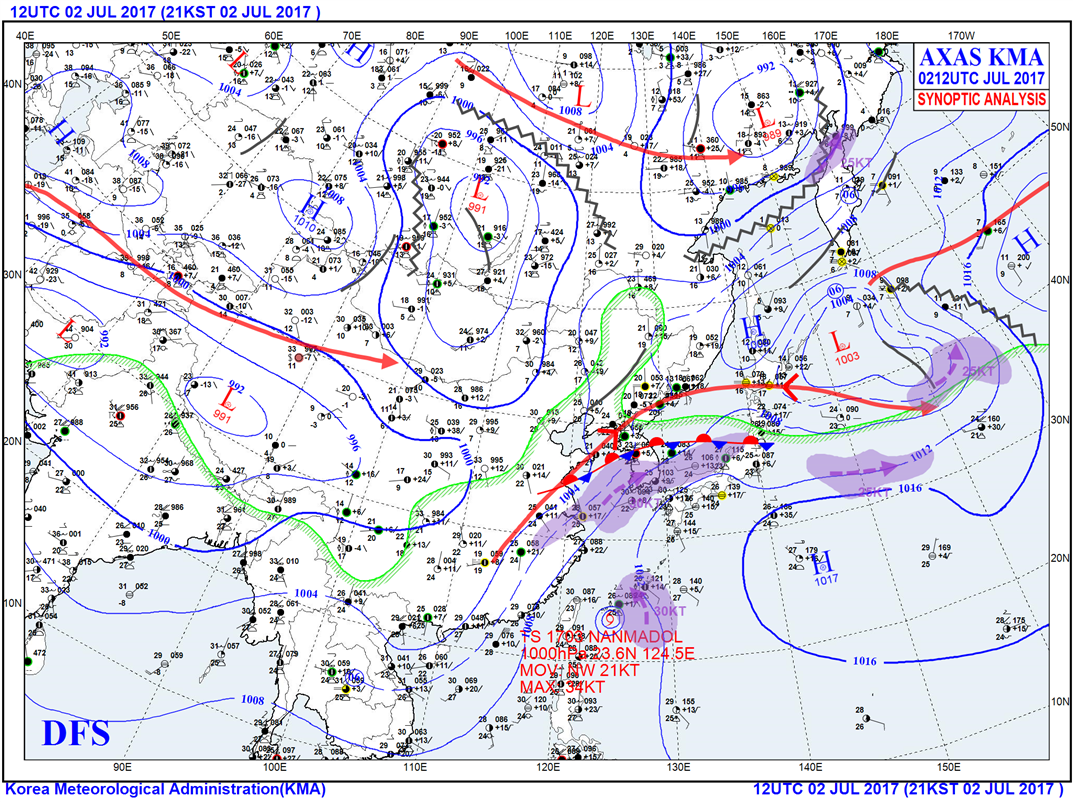
\includegraphics[width=0.8\linewidth]{surf_2017070212}
	\caption{기상청 지상일기도}
	\label{fig:surf2017070212}
\end{figure}

이와 비슷한 지도를 그리는 코드틑 다음과 같다.

\begin{code}[기상청 일기도모양 백지도]
	%	\begin{align}
	\begin{lstlisting}
	
	from mpl_toolkits.basemap import Basemap
	#python 
	import matplotlib.pyplot as plt
	import numpy as np
	
	# create new figure, axes instances.
	fig=plt.figure()
	ax=fig.add_axes([0.1,0.1,0.8,0.8])
	
	#loglat = [west,south,east,north]
	loglat = [90,0,180,62]
	clog = (loglat[2]+loglat[0])/2
	clat = (loglat[3]+loglat[1])/2
	
	# map projection.
	m = Basemap(llcrnrlon=loglat[0],llcrnrlat=loglat[1],\
	urcrnrlon=loglat[2],urcrnrlat=loglat[3],\
	resolution='l',projection='aea',lon_0=clog,lat_0=clat)
	
	m.drawcoastlines()
	m.drawcountries()
	m.fillcontinents()
	
	# draw parallels
	m.drawparallels(np.arange(0,90,10),labels=[1,1,0,0])
	# draw meridians
	m.drawmeridians(np.arange(-180,180,20),labels=[0,0,1,0])
	m.drawmeridians(np.arange(-180,180,10),labels=[0,0,0,1])
	
	plt.show()	
	\end{lstlisting}
	%		\end{align}
\end{code}

그 결과이다. 

\begin{figure}[h]
	\centering
	\includegraphics[width=0.8\linewidth]{weathermap01}
	\caption{기상청 일기도모양 백지도}
	\label{fig:weathermap01}
\end{figure}
	%\section{지구 온난화 모델링}

\subsection{Time-Stepping Naked Planet Model}\index{Time-Stepping Naked Planet Model}

\subsubsection{How the Model Works}\index{}

So the naked planet model is an energy balance model. We have energy coming in at some rate, and energy flowing out at a rate, which depends on the temperature of the planet. So the temperature and the heat content are related to each other by means of the heat capacity. Which is how many jewels it takes to raise the temperature of one square meter of the surface by one degree kelvin. And that number depends on the water depth, because the water is the sort of heat sink. So if we change this value to smaller value, you'll see the heat capacity change. Because I'm calculating the heat capacity as a function of the water depth. 
0:45
The incoming energy is from sunlight, and the albedo reflective energy is lost sort of off the top. And then outgoing is epsilon sigma T to the fourth. So you can calculate, at any given temperature, what the heat flux out will be. 
1:13
The way this works is that you want to keep track of the heat content of the planet. So you start out at a temperature of zero, the heat content will be zero. But then you have heat coming in and heat, not so much heat going out. And so you need to calculate how many joules of energy per square meter there are in that column, after a timestep of a certain duration. And once you have the heat content, you can calculate what the temperature is each timestep. You have to be careful about the length of the timestep. Because if you take a timestep that's too short for the water depth, it will become numerically unstable and blow up, very exciting. So what we do here is make the timestep shorter, let's try 50 years. 
2:09
That's better but, it's still looking a little jittery there. So, right, right, ten years and oh, you can't see the time scale is changing there so. If we change the timestep, we get the same number of time steps. But, each one goes longer so the number of years is longer. So now if we look at the Python script for this, we see it's very short. We define parameters up top. In both cases, it's real important to keep close track of the units. So I just have comments here for units. In the spreadsheet I have actual cells that I use to put units in just to keep it. It's much easier to debug if you can kind of keep it straight. And then, here is a loop that goes through the timesteps. And here are some plotting lines that use this Python library matplotlib to make the plot that we see. 


\subsubsection{방정식}\index{}

%The background for this material can be found in Sections 2 and 3 of Part I of this class. 
%Short version: Joules are units of energy; Watts are energy flow (J/s). The temperature of a planet is determined by balancing energy fluxes into and out of a planet. 

어느 행성에 단위 시간 당 입사되는 태양복사에너지($E_{in}$)\는 
\begin{equation}
{\rm E_{in} ~ = ~ \frac{L (1- \alpha)} {4}}
\label{eq:001}
\end{equation}
\와 같이 나타낼 수 있는데 여기서 ${\alpha}$\는 행성의 알베도이다. 그리고, 행성이 방출하는 복사에너지($E_{out}$)\는 
\begin{equation}
{\rm E_{out} ~ = ~ {\epsilon} ~ {\sigma} ~ T^4}
\label{eq:002}
\end{equation}
\로 나타낼 수 있는데 여기서 ${\epsilon}$\은 행성의 흑체율이고, ${\sigma}$\는 슈테판-볼쯔만 상수로 그 값은

\begin{equation}%[caption={code for map}, label=lst:Pythoncode]
{\rm \sigma ~ =~ \frac{2\pi^5~k^4}{15~c^3~h^3}~=~ 5.670400 \times 10^{-8}~ (J ~s^{-1}~m^{-2}~K^{-4})}
\end{equation}
이다. 

%The goal is to numerically simulate how the planetary temperature of a naked planet would change through time as it approaches equilibrium (the state at which it stops changing, which we calculated before). The planet starts with some initial temperature. The “heat capacity” (units of Joules / m2 K) of the planet is set by a layer of water which absorbs heat and changes its temperature. If the layer is very thick, it takes a lot more heat (Joules) to change the temperature. The differential equation you are going to solve is

행성의 표면 온도가 어떻게 평형을 이루는지 계산해 보자.
열용량(heat capacity)의 단위는 ${\rm J~ m^{-2}~K^{-1}$이고, 해양이 열을 흡수하여 행성의 온도가 변하는 것으로 가정하며 해양이 깊으면 열용량도 크다고 볼 수 있다.

\begin{equation}%[caption={code for map}, label=lst:Pythoncode]
{\rm \frac {dHeatContent} {dt} ~ = ~ \frac{ L~ (1 - \alpha )} {4} ~ - ~ \epsilon ~ \sigma ~ T^4}
\end{equation}


where the heat content is related to the temperature by the heat capacity.

\begin{equation}%[caption={code for map}, label=lst:Pythoncode]
{\rm T[K] ~=~ \frac{Heat~Content ~[J~m^{-2}]} {Heat~Capacity~[J~m^{-2}~K^{-1}]}}
\end{equation}


The numerical method is to take time steps, extrapolating the heat content from one step to the next using the incoming and outgoing heat fluxes, same as you would balance a bank account by adding all the income and subtracting all the expenditures over some time interval like a month. The heat content "jumps" from the value at the beginning of the time step, to the value at the end, by following the equation

\begin{equation}%[caption={code for map}, label=lst:Pythoncode]
{\rm HeatContent(t+1) ~=~ HeatContent(t) ~+~ \frac {dHeatContent} {dt} ~ TimeStep}
\end{equation}


This scheme only works if the time step is short enough that nothing too huge happens through the course of the time step.

Set the model up with the following constants:

\begin{lstlisting}%[caption={code for map}, label=lst:Pythoncode]

timeStep = 100           # years
waterDepth = 4000        # meters
L = 1350                 # Watts/m2
albedo = 0.3
epsilon = 1
sigma = 5.67E-8          # W/m2 K4

\end{lstlisting}



\begin{enumerate}
	\item Construct a time column, with the first time point being 0 and the rest of them going up by an increment, the time step, say 5 years. Make the time step a labeled number in a cell so you can easily change it later. 
	\item (The second time step value) = (the first value) + (the time step), and the third relative to the second and so on. If the amount of time per time step is in cell A1 for example, the formula to calculate step 2 from step 1 should point to A1 in an absolute way, using {\$A\$1}, so when you copy the formula downwards it keeps pointing to {\$A\$1} (as opposed to the previous time step pointer, without dollar signs, which shifts when you copy the cell downward. This saves retyping in formulas all the way down.
	\item Construct a column for the planetary temperature at each time step. Set the initial temperature (at time 0) to be some “initial condition” value (0 works).
	\item The heat capacity of the surface planet depends on the water thickness. Using the fact that 1 gram of water warms by 1 K with a calorie of heat, and the density of water, to calculate how many Joules of energy it takes to raise the temperature of 1 m2 of the surface, given some water depth in meters. Make the water depth a separate cell so you dial it up and down later.
	\item Create a column for the heat content of the surface layer at each time step. For the initial time, calculate the heat content from the temperature.
	\item Create a column for the incoming and outgoing heat fluxes at each time step. Base the incoming heat flux on the parameters solar constant (L), and albedo. The outgoing heat flux is a function of the temperature according to the Stefan-Boltzmann equation.
	\item Create yet another column where you combine the incoming and outgoing heat fluxes, and convert them from W/m2 to J/m2 timestep.
	\item Create a formula for the heat content at the second time point (the row below the first one), equaling the last heat content plus what came in and out in the previous timestep.
	\item Calculate the temperature at the second time step, from the heat content.
	\item Copy the formulas down to fill in the rest of the values at the second time step.
	\item Copy the second time step values down by 10 or 20 rows to create multiple time steps.
	\item Plot temperature versus time.
	\item Adjust the time step so that the temperature evolves smoothly (no numerical explosions) to an equilibrium value.
\end{enumerate}

이와 같은 방법으로 스프레드 시트를 이용하여 계산한 결과로 챠트를 그린 것이 \ref{fig:nakedchart01} 이다. 
\begin{figure}[b!]
	\centering
	\includegraphics[width=0.8\linewidth]{Pictures/naked__chart01}
	\caption{spread sheet를 이용하여 그린 챠트}
	\label{fig:nakedchart01}
\end{figure}

\newpage

\subsubsection{Python 이용}\index{}
\begin{enumerate}
	\item You’ll need to have numpy and matplotlib modules installed in your python programming environment, and in the first lines of your script import both of them.


\begin{lstlisting}%[caption={code for map}, label=lst:Pythoncode]

import numpy
import matplotlib.pyplot
\end{lstlisting}

	\item Define variables for the time step, the water depth, the heat capacity of the surface (units of J/m2 K), the solar constant, albedo, epsilon, and sigma. Since the energy influx doesn’t change through the simulation, calculate what that is (units W/m2).
	\item At the end of the simulation, in the code you submit for review, you will use

\begin{lstlisting}%[caption={code for map}, label=lst:Pythoncode]

matplotlib.pyplot.plot( time_list, temperature_list)
matplotlib.pyplot.show()
\end{lstlisting}

to create a plot of the temperature versus time. Create an array for time_list, initially [ 0 ] (a ‘list’ or array with one value in it, the number 0), and similarly for temperature_list. Set the initial temperature (maybe to 0 K, or whatever you like), and calculate the initial heat content (units of J/m2).

	\item Create a loop for time steps. Each step, calculate the outgoing heat flux, and the new heat content after taking up and giving off heat. Append the value of the time, and the temperature, from each step, at the end of the time and temperature lists.
	
Python tricks you may find useful:
a. arrayname.append( value ) to add another item to the end of a list
b. pow(T[-1],4) would raise the last temperature in the T list to the power of 4
My script for this model is 23 lines long.


\end{enumerate}


\subsubsection{Python 이용 해설}\index{}

Create a version of your python code which takes an argument from stdin for the number of time steps, using

\begin{lstlisting}%[caption={code for map}, label=lst:Pythoncode]

nSteps = int(input(""))
\end{lstlisting}

Note that the input statement differs between python 2.x and 3.x. Be sure to develop your python code using version 3 so it will run on the coursera servers. It's tricky, because python2 is the default "python" on most systems, but python3 is the version that is currently supported and is the future.

Also be sure to remove any plotting code (matplotlib) from your submission. Just insert a hash tag before the lines, to "comment it out".

\begin{lstlisting}%[caption={code for map}, label=lst:Pythoncode]

#import matplotlib
\end{lstlisting}


At the end of the simulation, have the code print out the temperature and the heat flux at that time, on a line by itself, using statements like

\begin{lstlisting}%[caption={code for map}, label=lst:Pythoncode]

print(TK[-1], heatOut)
\end{lstlisting}

Python interprets an index of -1 (in the square brackets) as the last element in the list, which will be the last temperature. When you run the code, the print statement should write a number all by itself on a single line of output, and that should be the only line of output from the code. Make sure it is in Kelvins.

For the heat flux, make sure that it is in units of Watts/m2, and make it current with the temperature. So, you'll calculate the heat flux at the beginning of a time step, then a new temperature. At the end of the simulation, calculate the heat flux one more time, using the temperature you got at the end of the last time step.

As a check, running the code with one time step gives

\begin{lstlisting}%[caption={code for map}, label=lst:Pythoncode]

python naked_planet.py
1
44.15624999999999 0.21555186906704765  
\end{lstlisting}

where you type in the first two lines, and the third comes from your code, and with two time steps

\begin{lstlisting}%[caption={code for map}, label=lst:Pythoncode]

python naked_planet.py
2
88.2722123292339 3.442540862251764     
\end{lstlisting}

There should only be two numbers output from the program, no text from a prompt (like "how many time steps would you like?", perfectly normal for interacting with humans but not with the grader). Any extraneous output will probably confuse the grader. The tolerances in the grader for temperatures are 2-3 degrees C, and for the heat fluxes, +- 0.1 W/m2.

\begin{code}[흑체 복사평형 온도]
	%	\begin{align}
	\begin{lstlisting}
	
import numpy
import matplotlib.pyplot

#variables
TimeStep = 20.0         # years
waterDepth = 4000.0      # meters
L = 1350.0               # Watts/m^2
albedo = 0.3             # No dim
epsilon = 1.0            # No dim
sigma = 0.0000000567     # W/m^2 K^4
Time = 0.                 #year
Teaperature = 0.00        #K
Heatcontents = 0.00         #J/m^2
Heatcapacity = 4200000. * waterDepth     #J/K m^2

#arrays
Teaperature_list=[]
Time_list=[]
Heatcontents_list=[]
HeatIN_list=[]
HeatOUT_list=[]

#calculate
for i in range(0,100):
Time_list.append(Time)
Teaperature_list.append(Teaperature)
Heatcontents_list.append(Heatcontents)
HeatIN = L*(1-albedo)/4
HeatOUT = epsilon * sigma * Teaperature**4
HeatIN_list.append(HeatIN)
HeatOUT_list.append(HeatOUT)
Heatcontents = Heatcontents + ((HeatIN - HeatOUT) * TimeStep * 265.2425 * 24 * 3600)
Teaperature = Heatcontents / Heatcapacity
Time = Time + TimeStep

#draw chart
matplotlib.pyplot.plot(Time_list, Teaperature_list)
matplotlib.pyplot.show()
	
	\end{lstlisting}
	%		\end{align}
\end{code}

\subsubsection{Quiz}\index{}
Adapt the code to simulate a dry planet, like Mars. The effective heat capacity of a solid surface is much smaller than that of an ocean, because heat diffuses very slowly in solids compared to fluid mixing in liquids. On time scales of a few years, heat penetrates a meter or a few meters into a soil column. Approximate a solid surface by changing the depth of the water in your model to 1 meter.

The trick here is that you will have to take smaller time steps to keep the numerical method from blowing up. A good way to see what's going on is to decrease the ocean depth in stages. Start with 2000 meters, then 1000, then 100, then 10, then 1. Each time you'll have to make the time step shorter, and if it's too long you'll see the numerics to crazy.

What is the longest time step you can take for model stability, using a water depth of 1 m?



Change the initial temperature to 400 Kelvins. What is the value of the outgoing emission flux at time 0, within a tolerance of 1 Watt/m2?



Set the ocean depth to 4000 meters and the time step to 10 years. Keep he initial temperature 400 K from the last problem. What is the outgoing heat flux after 100 years?



What is the outgoing heat flux, in Watts/m2, after 2000 years? (Your model should be in equilibrium at this point).




\subsection{Iterative Runaway Ice-Albedo Feedback Model}\index{Iterative Runaway Ice-Albedo Feedback Model}

\subsubsection{How the Model Works}\index{}

The second model you're going to be working on is an iterative model of the Ice-Albedo Feedback and how it affects the temperature of the Earth. So instead of stepping through the time in this model, we're going to be making successive guesses of what the right answers are and the guesses will converge and get closer. You get the same answer every time you guess as you get towards the end, so it's a fundamentally different kind of calculation. 
0:30
So the idea is that if planet is cold, it will have ice and snow, which is very reflective, and so that will reflect incoming energy. Whereas if the planet is warmer there's none of that stuff, and so the sunlight is absorbed more effectively. So if this is the energy balance of the planet, here is the incoming solar [COUGH], and here is the outgoing infrared which is a function of the temperature of the planet. 
1:00
The Albedo here kind of comes off the top of the incoming solar, gets reflected away, rather than absorbed and this is a function of ice, which is a function of temperature. 
1:12
So, the calculation gives you a linear function of temperature to describe the latitude, that ice will form on a planet, so the colder it is, the more the ice can be found closer and closer to the equator. And another equation is given with the Albedo as a function of temperature, and again, you're going to fit a straight line to the data that you're given. And so the idea is to start with a guess for the Albedo, and then using that Albedo, calculate the temperature. 
1:55
And then from this temperature get another guess for the Albedo, and then go back for another temperature, and then back and forth, back and forth, iterating between Albedo and temperature. This is what the snowball code looks like in Python, it has one loop going up and the other loop going down where we're looping over different values of the solar constant. So, for going down we start with a high solar constant, and so, the temperature is warm and the Albedo is probably ice free and that's true for many of these different values of L. But then, at some point you cross a value of L where it starts to freeze a little bit and so then it takes a few iterations, this is the number of iterations here for the temperature and Albedo to stop changing. And then at some point there's a critical solar constant value at which all of a sudden the feedbacks run all the way to the equator, and the temperatures 
3:10
go all the way down, the Earth gets covered with ice like a snowball. 
3:17
So if i change the plot type here and run that again, we can see. We are now looking at the equilibrium temperature after the iterations as a function of the solar constant in this dimension. And the reason why this isn't a simple line is because there is hysteresis in the system, if you start up here from an ice-free state and you cool the sun down in this dimension, the temperature, of course, gets colder but you don't start to get any ice until you reach an insulation that's sort of here, solar sunlight rate insulation. And then at some point you drop down into the snowball make it colder, it's just ice frozen all the way anyways, so just the sun effect here. But then as you warm it back up, the ice sheet is able to perpetuate its own existence by reflecting sunlight back to space. And so to get out of the snowball, it takes considerably more work, than it took to get- than it took sort of coolness to get into it, this is what we call hysteresis, or path dependence. 
Downloads

Lecture Videomp4
Subtitles (English)
WebVTT
Transcript (English)


\subsubsection{T와 Ice ltitude and Albedo 파라메타}\index{}

The first part of this calculation is a pair of regressions to calculate the slope and intercept for two linear functions: one is the latitude to which there will be snow and ice on the surface (lower latitudes, closer to the equator, when it’s colder), and the second is the overall albedo from ice that you will get at that temperature. You are looking for functions Ice latitude = m1 * T + b1 and albedo = m2 * T + b2. The regression is probably easier to do in a spreadsheet, either using a built-in least-squares function, or by setting up a trial function with values of m and b in cells that you tweak by hand, and compare the resulting line in a plot with the plotted values of the data.

Use the following table to derive functions to describe the ice latitude and the albedo from the ice as a function of the mean planetary top-of-atmosphere (radiating) temperature.Assume that the functions are linear (which they pretty much are in this table).

Mean Planetary Temperature	Ice Latitude	Planetary Albedo
265	75	0.15
255	60	0.25
245	45	0.35
235	30	0.45
225	15	0.55
215	0	0.6타

The functions should be in slope / intercept form, as in ice_latitude = m1 * T + b1 and albedo = m2 * T + b2.

\subsubsection{스프레드시트 이용}\index{}
It is possible for a spreadsheet to do all the calculations that the Python version of this exercise will do, but it's starting to get cumbersome. You will want to do about 40 values of L, and each value of L will require 100 iterations or so before we can be sure that the process has converged. In a spreadsheet, typically, all of the iterations would be saved in separate cells. (It is also possible to use built-in iteration functions in some spreadsheets, which might avoid this problem). A sensible solution might be to restrict the spreadsheet to working on a single value of L, which will be useful for checking and debugging your Python script, and then leave the power-crunching of lots of different values of L to the script.

Set a value of L as a labelled number in a cell (with units!). You'll also need an initial guess for the albedo, and maybe values for epsilon and sigma would be useful. Also make cells with the slope and intercept values for your parameterized fits to the albedo and ice-latitude functions of temperature you derived in the first part.

Each iteration will take a separate line in the sheet. The left-most column should contain an iteration number. Start with 1 in the top cell and then write a formula adding 1 to that, in the cell below it. Then copy that formula down until you reach 100. (This can be done in one big copy operation).

The next column will be temperature guesses, and the third albedos.

Solve for the first temperature guess assuming the initial guess for the albedo. Then use that temperature to calculate a new albedo, the second guess, below the first. The albedo depends on the temperature in your parameterization, but don’t allow your parameterization to extrapolate to values outside the range in the data, that is, higher than a value of 0.7, or lower than a value of 0.15. You can use the MIN and MAX functions of the spreadsheet to limit the values to the reasonable range. Then, from that albedo second guess, calculate a second guess for the temperature. Construct these formulas so that they can be copied down to fill out the rest of the iterations.

Make a plot of temperature versus iteration number to see how many iterations it takes before it converges. A value of L to try is 1250 W/m2, with an initial guess for the albedo of 0.15.

\subsubsection{Python 이용}\index{}

As in the last problem, begin by importing library packages that we'll need, for messing with lists (arrays), and for plotting.

\begin{lstlisting}%[caption={code for map}, label=lst:Pythoncode]

import numpy
import matplotlib.pyplot
\end{lstlisting}

Define and initialize variables for the number of iterations, the M and B values from the albedo and ice line regressions from Part I, and for epsilon and sigma. Also set up variables for the range of L values over which you are going to do the calculation

\begin{lstlisting}%[caption={code for map}, label=lst:Pythoncode]

LRange = [ 1200, 1600 ]
\end{lstlisting}
Each pass over the range in L values requires two nested loops, the outer one over values of L, and the inner one for the iterations. Start with a cooling sweep from the highest L value

\begin{lstlisting}%[caption={code for map}, label=lst:Pythoncode]

L = LRange[1]
albedo = 0.15
while L > LRange[0]-1:
blah blah blah
L = L - 10
LRange = [ 1200, 1600 ]
\end{lstlisting}

where you'll want to replace the pseudo-code ("blah blah blah") with another, inner, loop, in which you iterate, finding new values for albedo, then T, then albedo again, until the T and albedo values you wind up with are consistent with each other (it "converges"). Before you begin any of the iterations, set the albedo to 0.15, and for each iteration (for each L), set the initial albedo for your iteration equal to the value you got for the converged albedo from the last iteration. Then go back and forth, calculating T from that initial albedo, then albedo from that T (limited to the range 0.15 to 0.65), back and forth each time. In contrast to the spreadsheet, there is not much penalty for taking lots of iterations; it doesn’t get ungainly but just runs slower.

Copy this loop-within-a-loop into a second pass in your code, then modify it to start from the lowest value of L (LRange[0]), and work back up to LRange[1]. Use the same strategy for albedo: for the initial guess, use the final value from the last set of iterations (the last L value).

For plotting, build three options. It's easiest to just have one plot at a time, so define a variable plotType which contains a string telling what kind of plot you want to see.

As the code runs, it should fill up two lists, which we can call x and y. What you put into x and y as the run progresses depends on the value of the variable plotType.

Initialize the lists with

\begin{lstlisting}%[caption={code for map}, label=lst:Pythoncode]

x_list = []              # an empty list
y_list = []
\end{lstlisting}

then each time you want to add something to the list, append the values to the end of the list, as, for example,

\begin{lstlisting}%[caption={code for map}, label=lst:Pythoncode]

x_list.append( L )
\end{lstlisting}

The three options for plots types I'd recommend are:

Option 1: the temperature after the iterations are done for each value of L, plotted as a function of L, for the entire series of calculations as L first sweeps down and then back up again. This plot will show the hysteresis in the ice albedo feedback, how there are multiple steady states for some intermediate values of L (including our own!).

Option 2: the temperature each iteration, for each value of L, plotted as a function of the iteration number, for the first sweep over L values, when each L is lower than the last. The trick here is to insert values of numpy.nan (stands for Not A Number) into the x and y arrays at the end of each iteration loop, when the number of iterations resets from the maximum number (for the last L value) to 0 (for the next L value). When matplotlib makes a plot of these lists, we don't want it to draw a line connecting these. It makes the plot messy and doesn't mean anything. So the nan value tells the plot library not to draw that line.

Option 3: same as option 2 but for the second sweep through the range in L, when the sun is getting hotter as you go through.

There are other interesting things you might want to see, such as the albedo or the ice latitude in any of these plot types. To see the ice latitude as a function of L, change the y_list.append( ) statement to append the ice latitude rather than the temperature.

Then, when all the calculations are done,


\begin{lstlisting}%[caption={code for map}, label=lst:Pythoncode]

matplotlib.pyplot.plot( x, y )
matplotlib.pyplot.show( )
\end{lstlisting}

will create a plot of your results.

My script required about 60 lines of python code. New python functions you may find useful include min() and max().


\subsubsection{Quiz}\index{}


On the downward sweep through L (getting colder each time), What is the maximum value of the solar constant, L, in units W/m2, for which the planet freezes all the way to the equator? (Make sure you have enough iterations to see that your temperature and albedo have reached equilibrium). The tolerance in the grader is a range of 20 W/m2.


Now on the upward sweep through the range in L, at some critical L value (in Watts/m2), the temperature jumps up to a higher value. What value of L do you get for this sudden transition, as the snowball melts? The tolerance in the grader is a range of 50 W/m2.



\subsection{A Simple 1-D Ice Sheet Flow Model}\index{A Simple 1-D Ice Sheet Flow Model}

Ice Sheet Dynamics

Ice flows like extra-thick molasses, downhill. The shape of the ice sheet (altitude versus distance across) is determined by the relationship between ice surface slope and the flow rate of the ice.


\subsubsection{How the Model Works}\index{}
The Ice Sheet Model is formulated in one dimension, a horizontal dimension and so we have snow that's accumulating all the way across this dimension. And as the ice gets thicker and thicker you get a slope at the ice surface which drives a pressure gradient which drives flow in both directions. The flow is always going sort of down hill. The flow is given by the surface slope, the change in elevation over the change in x of the slope of the surface there, times some constant, which will be given to you. So we're going to solve this problem numerically by breaking it up into pieces, and each of those pieces, we're going to call a grid cell. And so there will be some number of grid cells across the domain, and each grid cell has an elevation which is defined in the center of the cell and so 
1:11
the slope in the elevation would be the difference in x divided by the difference in x so the slope would be sort of between two adjacent points like that. And then there are flows defined in the domain as well going between one grid cell and another. So the flows are actually defined on the cell faces, whereas the elevations are in the cell centers. Another crucial part of this problem is the boundary condition. We have to keep it zero at the edges where the ice is flowing into the water. We're not going to let it build up higher than that. And that sort of controls the whole domain of the ice sheet. And the way that boundary condition manifests itself in a grid like this is to have some extra grid points, some sort of ghost 
2:00
grid cells on both sides, where you specify that the elevation has to be equal to zero at all times. So you have to treat those cells special. >> So this is what the Ice Sheet Model looks like in my spreadsheet version. I have, as usual, some parameters up at the top govern things, so I can change stuff on the fly and have it reflected everywhere, including units. So time step in years, 100 years. 
2:30
I have the time steps on rows going down here. So, this is the time in years, and this is going up to 23 thousand years and then we have to have elevations and we have to have flows. So I have elevations, I have ten of those, and then I have two grid cells at the edges, and then the flows go between those elevations. So, can see right 
3:02
here there's difference in elevation 
3:07
with x and that means that you get a flow there. 
3:13
In Python, this is what the code looks like. 
3:18
It's a short little code, very easy, and this is what it looks like when it runs. So now we're making the Python make a new plot every single time step and so you can see how the elevation is changing through time. 
3:38
We change the number of grid points. Say we make 20 grid points instead of ten. 
3:50
We get a smoother curve but we have to be careful about the time step. 
3:55
Because as you make the grid points closer together, you need to make the time step 
4:01
shorter, or else something like that happens where it just blows up. Decrease the time step. 
4:10
In general, a factor of two change in the size, factor of two change in the time step should work. More or less, we'll see. 
4:24
Taking longer for the action to happen here, because we're taking shorter time steps. 

\subsubsection{Model Formulation}\index{}
Ice flows, like any other fluid, only very slowly, due to its high viscosity. The force driving the flow is differences in pressure in the interior of the ice, which arise from differences in the elevation of the ice surface. If you make a pile of ice, it's like a pile of molasses, in that it will flow outward and flatten itself out.

The model is formulated in one dimension, on a horizontal grid. Start with 10 grid cells. Let them span a horizontal distance of 1000 km, or 10^6 meters. Each grid cell will have an elevation of ice. Flow between adjacent cells depends on the difference between their elevations. Snow falls equally on all grid cells. Also, vitally important to this type of problem, is a boundary condition. We'll assume that the ice sheet is confined to a landmass like Greenland or Antarctica, so that the thickness of the ice at the boundaries has to be zero. Ice flows into the ocean and disappears, both in reality and in our model.

In the real world, the ice surface might slope upward in some direction throughout what we are calling a grid point. The elevation we are keeping track of might be the average elevation within that region. For the best approximation to reality from our simple grid, let's specify that the elevation of a cell applies in the center of the cell. In contrast, the flow between the cells can most sensibly be defined on the cell boundaries. This combination is called a "staggered" grid, where all of the variables are not defined in the same places. Including flows from the grid cells on the edges of the ice sheet, there will be 11 flows among the 10 grid cells of the simulation. My suggestion is to draw a cartoon with your grid, showing the index numbers of the two variables. It can get confusing.

The confusion is compounded by the boundary condition (the ice vanishes when it hits the ocean). The easiest way is to define two extra grid cells for the elevations, and keep them always set to a value of 0. This means that you will have nX+1 = 11 values in the list of fluxes (between each of the 10 boxes), and nX+2=12 values in the list for elevations, to contain the "ghost" cells that will always have 0 elevation.

The model will step forward in time, using a time step of 100 years. It will begin to rise uniformly, but the elevations at the edges will be eroded by flow to the ocean. Eventually it will reach a steady state, where snowfall in each grid cell is balanced by flow from the grid cell, which is all determined by the slope of the ice surface.

Parameter Settings

Set the following parameter values

\begin{lstlisting}%[caption={code for map}, label=lst:Pythoncode]

nX = 10                # number of grid points
domainWidth = 1e6      # meters
timeStep = 100         # years
nYears = 50000         # years
flowParam = 1e4        # m horizontal / yr
snowFall = 0.5         # m / y
\end{lstlisting}

Initialize the elevations to zero.

Calculate the flows as

\begin{lstlisting}%[caption={code for map}, label=lst:Pythoncode]

flow[ix] = ( elevation[ix] - elevation[ix+1] ) / dX * flowParam  * \
( elevation[ix]+elevation[ix+1] ) / 2 / dX
\end{lstlisting}

where the first incidence of the dX variable is to calculate the gradient in elevation, and the second one corrects for the aspect ratio of the grid cell, how much horizontal flow translates into vertical elevation. Be sure that you have the indexing right for your implementation of the staggered grid, and be sure to get the sign right, so that flow from the first cell in the list to the second would be defined as positive.

Then update the elevations by adding ( snowFall + flow[ix-1] - flow[ix] ) * timeStep.

Repeat the cycle, calculating flows, then taking time steps in the elevation. Watch the ice sheet grow in, through time, to its equilibrium shape, which will be determined by the math in the equations described above

\subsubsection{스프레드 시트 이용}\index{}

I always find it useful to take some space at the top of a spreadsheet for model parameters, like the time step etc. I use three cells for each parameter, one for the name, one for the units (years, in this case), and a third for the numeric value.

Beginning below the parameter area, make a column of time values, with a step equal to the time step. You'll want to see many thousands of years.

Set up an array of 12 columns alongside the time column, for the elevations. Fill the first and 12th column with zeros. Fill the first row with zeros.

Set up another array of 11 columns to hold the flow rates. Create the formula for the first flow rate (leftmost, topmost) by referencing the contents of two elevation values, and parameters like the flow constant. Use relative addressing to point to elevations, and absolute addressing to point to parameters, so that you can copy the formula you create across and down across the entire block of flow values.

Go back to the elevation array, and write a formula to update the elevations in the first grid cell (leftmost, topmost). The ice in that cell in year 100 will be equal to that in year 0, plus snowfall, plus flow coming in from the left (which will be positive if it's coming into this cell), minus flow going out to the right. Because the flow is actually going to the left in this first cell, the flow number you'll be using should be negative.

Use relative and absolute addressing as you did with the flow formula so that you can copy the elevation formula to the rest of the elevation block.

Make a plot of the elevation as a function of distance at some time slice, to see the shape of the ice sheet as it evolves toward its steady state.


\subsubsection{Python 이용}\index{}

The advantage of a scripting tool like python for this calculation is that it's no trouble at all to do a longer calculation -- we don't have to save all the intermediate values of all the variables.

Initialize the elevations and flows


\begin{lstlisting}%[caption={code for map}, label=lst:Pythoncode]

elevations = numpy.zeros(nX+2)
flows = numpy.zeros(nX+1)
\end{lstlisting}

Create a time loop which first calculates flows (by looping over the horizontal grid points, using the current values of the elevations), then takes a time step for the elevations (looping over the horizontal grid again).

The plotting infrastructure in Python, matplotlib, can be used to create a cool animation of the evolving ice sheet. Before starting the time loop, set things up using


\begin{lstlisting}%[caption={code for map}, label=lst:Pythoncode]

fig, ax = matplotlib.pyplot.plot.subplots()
ax.plot(elevations)
ax.set_ylim([0,plotLimit])
matplotlib.pyplot.plot.show(block=False)
\end{lstlisting}

where the block=False flag tells Python to throw the plot on the screen then keep moving. Within the time loop, issue the commands

\begin{lstlisting}%[caption={code for map}, label=lst:Pythoncode]

ax.clear()
ax.plot( elevations )
matplotlib.plot.show( block=False )
matplotlib.pyplot.pause(0.001)
fig.canvas.draw()
\end{lstlisting}

These commands will update the plot to show the latest elevations, and then keeps moving.


\subsubsection{Quiz}\index{}
Set up the code to run for 25,000 years of simulated time. Does the code reach equilibrium by the end of this time?  
yes / no

What elevation does the ice sheet reach, in meters?


What is the longest value of the time step that you can use, which still looks like the solution you got above?


When the model uses a time step which is just a bit too long, what happens to the run?

- It crashes immediately
- It starts up unstable (with oscillating values) then settles down for the equilibrium part of the simulation.
- It runs OK while it's spinning up but gets twitchy and blows up after it reaches equilibrium

If you double the snowfall rate, the equilibrium elevation of the ice sheet

 - doubles
 - more than doubles
 - less than doubles
 - stays the same

\subsection{A 2-D Gridded Shallow Water Model}\index{A 2-D Gridded Shallow Water Model}
Pressure, Rotation, and Fluid Flow

Planetary rotation and fluid flow were explained in Part I of this class, Unit 6, on Weather and Climate.

\subsubsection{How the Model Works}\index{}
0:05
The shallow-water equations are not necessarily called that because water has to be shallow, but because the flows are the same at all water depths. So we're doing the calculation of water flow that is independent of water depth where you don't have different flows. You have to maintain different grid cells in the vertical, you just need a lattice of grid cells in two dimensions in the horizontal. So this is what that grid looks like, so this is latitude and longitude. And each grid cell has an elevation of water level height which is defined, just like in the ice sheet model, it's defined in the cell centers. And then there are flows between the cells, which are like in the ice sheet model designed on the cell edges. So the grid could look like h00, h01, h02, and then v velocities, which are the north south velocities defined on the south faces there are now four of them as opposed to the three elevations. Just like in the ice sheet model, you have to worry about the boundaries. Now the north and south boundaries, we are going to say that there is a wall there so. These flows are both going to all equal zero across that wall and that wall. In the horizontal dimension there will be two options you're going to build into your code. One is to put walls there which means that you'll be setting these velocities, these u values to be zero. And the other is to have it wrap around in which case, you have stuff can flow out one side and it would just flow in the other side. So the way that you calculate the evolution of the elevation of the surface is by tracking the flows coming and going out the boundaries. So dU/dX, that's saying you have, more flowing in this side than that side. That would give you a value du dx that would actually be decreasing as you go this way. And so the negative of that multiplied by the aspect ratio. Tells you how much of this water is going to be piling up and making this box get deeper. 
2:31
So to accomplish this model, you are going to be given a template which has a lot of the overhead dealt with for you already like that makes the animation and what not. So this is what that template looks like. There's some stuff here at the top that you can play with after you get everything going. 
2:52
Some stuff here that you probably won't need to change. It's just sort of set up and then here is the main time stepping subroutine, and there are instructions for how to write Python loops to calculate the derivatives. The DUDX and the VDDY and things like that. In this loop, so you just need to flesh out this loop here. As the template comes initially, it's simplest to de-bug a thing like this when it's got a really small grid. So, this is what the thing will look like, just in the three by three grid. And the colors are the elevations and the arrows are the flows defined at the cell faces, like I said. And this particular simulation starts out with a big tower of water in the middle. And you get wild flow initially but then it settles down to a geostrophic balance where the rotation is balancing the pressure gradient sort of sideways. Three by three isn't very exciting so if we expand that to a bigger grid so there's the initial transient waves going all over the place. But then it settles down, and you get this sort of rotation going around the perturbation, this high pressure in the center. And this wave will tend to drift to the west. Because the rotation of the planet in higher latitudes is faster than the rotation rate in lower latitudes and that's set in this model. And so that tends to make raspy waves like this drift toward the west. So you can see this cell is getting redder and redder than that one as this peak is sort of going to slowly move across this grid, toward the West. I should say that this is a very, very small ocean. And it's got a very big degree of rotational change between the lower part latitude and the high latitude here. So it's like a small ocean on a small planet, but with the limited power of Python, we have to do what we can to make things run quickly. 
5:21
Here's another trick that the shallow water circulation code can do. In this case, you have winds that are blowing in this direction toward the west in the lower 
5:35
half of this domain and in the upper half the winds are blowing toward the east. And with the rotation what that does is it causes water to pile up in the center of this gyre. And once this water piles up, that pressure gradient actually starts to drive the flow around the gyre. So it's going the way the wind would tell it to go, but it's going there because the pressure gradient in the water is telling it to, not because the wind is telling it to. These arrows arise as this pressure difference in the water arises. And then this is like a giant Rossby wave, it's drifting to the west. And what that does in this case where you have walls at the east and west boundaries is it tends to lead to an intense flow on the Westward boundary. This is called Westward intensification and it's responsible for the Gulf stream and the Kuroshio and other Western boundary currents around the world that are very intense for this dynamical reason. 

\subsubsection{Model Description}\index{Model Description}

\begin{lstlisting}%[caption={code for map}, label=lst:Pythoncode]

"""
The first section of the code contains setup and initialization 
information.  Leave it alone for now, and you can play with them later 
after you get the code filled in and running without bugs.  
"""

# Set up python environment.  numpy and matplotlib will have to be installed
# with the python installation.

import numpy
import matplotlib.pyplot as plt
import matplotlib.ticker as tkr
import math

# Grid and Variable Initialization -- stuff you might play around with

ncol = 3         # grid size (number of cells)
nrow = ncol

nSlices = 2         # maximum number of frames to show in the plot
ntAnim = 1          # number of time steps for each frame

horizontalWrap = True # determines whether the flow wraps around, connecting
# the left and right-hand sides of the grid, or whether
# there's a wall there. 
interpolateRotation = True
rotationScheme = "PlusMinus"   # "WithLatitude", "PlusMinus", "Uniform"

# Note: the rotation rate gradient is more intense than the real world, so that
# the model can equilibrate quickly.

windScheme = ""  # "Curled", "Uniform"
initialPerturbation = "Tower"    # "Tower", "NSGradient", "EWGradient"
textOutput = False
plotOutput = True
arrowScale = 30

dT = 600 # seconds
G = 9.8e-4 # m/s2, hacked (low-G) to make it run faster
HBackground = 4000 # meters

dX = 10.E3 # meters, small enough to respond quickly.  This is a very small ocean
# on a very small, low-G planet.  

dxDegrees = dX / 110.e3
flowConst = G  # 1/s2
dragConst = 1.E-6  # about 10 days decay time
meanLatitude = 30 # degrees

# Here's stuff you probably won't need to change

latitude = []
rotConst = []
windU = []
for irow in range(0,nrow):
if rotationScheme is "WithLatitude":
latitude.append( meanLatitude + (irow - nrow/2) * dxDegrees )
rotConst.append( -7.e-5 * math.sin(math.radians(latitude[-1]))) # s-1
elif rotationScheme is "PlusMinus":
rotConst.append( -3.5e-5 * (1. - 0.8 * ( irow - (nrow-1)/2 ) / nrow )) # rot 50% +-
elif rotationScheme is "Uniform":
rotConst.append( -3.5e-5 ) 
else:
rotConst.append( 0 )

if windScheme is "Curled":
windU.append( 1e-8 * math.sin( (irow+0.5)/nrow * 2 * 3.14 ) ) 
elif windScheme is "Uniform":
windU.append( 1.e-8 )
else:
windU.append( 0 )
itGlobal = 0

U = numpy.zeros((nrow, ncol+1))
V = numpy.zeros((nrow+1, ncol))
H = numpy.zeros((nrow, ncol+1))
dUdT = numpy.zeros((nrow, ncol))
dVdT = numpy.zeros((nrow, ncol))
dHdT = numpy.zeros((nrow, ncol))
dHdX = numpy.zeros((nrow, ncol+1))
dHdY = numpy.zeros((nrow, ncol))
dUdX = numpy.zeros((nrow, ncol))
dVdY = numpy.zeros((nrow, ncol))
rotV = numpy.zeros((nrow,ncol)) # interpolated to u locations
rotU = numpy.zeros((nrow,ncol)) #              to v

midCell = int(ncol/2)
if initialPerturbation is "Tower":
H[midCell,midCell] = 1
elif initialPerturbation is "NSGradient":
H[0:midCell,:] = 0.1
elif initialPerturbation is "EWGradient":
H[:,0:midCell] = 0.1

"""
This is the work-horse subroutine.  It steps forward in time, taking ntAnim steps of
duration dT.  
"""

def animStep():    

global stepDump, itGlobal

# Time Loop
for it in range(0,ntAnim):

# Here is where you need to build some code

# Encode Longitudinal Derivatives Here

# Encode Latitudinal Derivatives Here

# Calculate the Rotational Terms Here

# Assemble the Time Derivatives Here

# Step Forward One Time Step

# Update the Boundary and Ghost Cells

#   Now you're done

itGlobal = itGlobal + ntAnim

def firstFrame():
global fig, ax, hPlot
fig, ax = plt.subplots()
ax.set_title("H")   
hh = H[:,0:ncol]
loc = tkr.IndexLocator(base=1, offset=1)
ax.xaxis.set_major_locator(loc)
ax.yaxis.set_major_locator(loc)
grid = ax.grid(which='major', axis='both', linestyle='-')
hPlot = ax.imshow(hh, interpolation='nearest', clim=(-0.5,0.5))   
plotArrows()
plt.show(block=False) 

def plotArrows():
global quiv, quiv2
xx = []
yy = []
uu = []
vv = []
for irow in range( 0, nrow ):
for icol in range( 0, ncol ):
xx.append(icol - 0.5)
yy.append(irow )
uu.append( U[irow,icol] * arrowScale )
vv.append( 0 )
quiv = ax.quiver( xx, yy, uu, vv, color='white', scale=1)
for irow in range( 0, nrow ):
for icol in range( 0, ncol ):
xx.append(icol)
yy.append(irow - 0.5)
uu.append( 0 )
vv.append( -V[irow,icol] * arrowScale )
quiv2 = ax.quiver( xx, yy, uu, vv, color='white', scale=1)

def updateFrame():
global fig, ax, hPlot, quiv, quiv2
hh = H[:,0:ncol]
hPlot.set_array(hh)
quiv.remove()    
quiv2.remove()
plotArrows()
fig.canvas.draw()
print("Time: ", math.floor( itGlobal * dT / 86400.*10)/10, "days")

def textDump():
print("time step ", itGlobal)    
print("H", H)
print("dHdX" )
print( dHdX)
print("dHdY" )
print( dHdY)
print("U" )
print( U)
print("dUdX" )
print( dUdX)
print("rotV" )
print( rotV)
print("V" )
print( V)
print("dVdY" )
print( dVdY)
print("rotU" )
print( rotU)
print("dHdT" )
print( dHdT)
print("dUdT" )
print( dUdT)
print("dVdT" )
print( dVdT)

if textOutput is True:
textDump()
if plotOutput is True:
firstFrame()
for i_anim_step in range(0,nSlices):
animStep()
if textOutput is True:
textDump()
if plotOutput is True:
updateFrame()
#print(dHdT[0,1])


\end{lstlisting}

\subsubsection{....}\index{}
\subsubsection{....}\index{}
\subsubsection{....}\index{}
\subsubsection{....}\index{}
\subsubsection{....}\index{}


\subsubsection{....}\index{}


\begin{lstlisting}%[caption={code for map}, label=lst:Pythoncode]

\end{lstlisting}

\subsubsection{....}\index{}
\subsubsection{....}\index{}
\subsubsection{....}\index{}
\subsubsection{....}\index{}
	%%----------------------------------------------------------------------------------------
%	PART
%----------------------------------------------------------------------------------------
\usechapterimagetrue
\part{Part One}

%----------------------------------------------------------------------------------------
%	CHAPTER 1
%----------------------------------------------------------------------------------------

\chapterimage{chapter_head_2.pdf} % Chapter heading image

\chapter{Text Chapter}

\section{Paragraphs of Text}\index{Paragraphs of Text}

\lipsum[1-7] % Dummy text

%------------------------------------------------

\section{Citation}\index{Citation}

This statement requires citation \cite{book_key}; this one is more specific \cite[122]{article_key}.

%------------------------------------------------

\section{Lists}\index{Lists}

Lists are useful to present information in a concise and/or ordered way\footnote{Footnote example...}.

\subsection{Numbered List}\index{Lists!Numbered List}

\begin{enumerate}
\item The first item
\item The second item
\item The third item
\end{enumerate}

\subsection{Bullet Points}\index{Lists!Bullet Points}

\begin{itemize}
\item The first item
\item The second item
\item The third item
\end{itemize}

\subsection{Descriptions and Definitions}\index{Lists!Descriptions and Definitions}

\begin{description}
\item[Name] Description
\item[Word] Definition
\item[Comment] Elaboration
\end{description}

%----------------------------------------------------------------------------------------
%	CHAPTER 2
%----------------------------------------------------------------------------------------

\chapter{In-text Elements}

\section{Theorems}\index{Theorems}

This is an example of theorems.

\subsection{Several equations}\index{Theorems!Several Equations}
This is a theorem consisting of several equations.

\begin{theorem}[Name of the theorem]
In $E=\mathbb{R}^n$ all norms are equivalent. It has the properties:
\begin{align}
& \big| ||\mathbf{x}|| - ||\mathbf{y}|| \big|\leq || \mathbf{x}- \mathbf{y}||\\
&  ||\sum_{i=1}^n\mathbf{x}_i||\leq \sum_{i=1}^n||\mathbf{x}_i||\quad\text{where $n$ is a finite integer}
\end{align}
\end{theorem}

\subsection{Single Line}\index{Theorems!Single Line}
This is a theorem consisting of just one line.

\begin{theorem}
A set $\mathcal{D}(G)$ in dense in $L^2(G)$, $|\cdot|_0$. 
\end{theorem}

%------------------------------------------------

\section{Definitions}\index{Definitions}

This is an example of a definition. A definition could be mathematical or it could define a concept.

\begin{definition}[Definition name]
Given a vector space $E$, a norm on $E$ is an application, denoted $||\cdot||$, $E$ in $\mathbb{R}^+=[0,+\infty[$ such that:
\begin{align}
& ||\mathbf{x}||=0\ \Rightarrow\ \mathbf{x}=\mathbf{0}\\
& ||\lambda \mathbf{x}||=|\lambda|\cdot ||\mathbf{x}||\\
& ||\mathbf{x}+\mathbf{y}||\leq ||\mathbf{x}||+||\mathbf{y}||
\end{align}
\end{definition}

%------------------------------------------------

\section{Notations}\index{Notations}

\begin{notation}
Given an open subset $G$ of $\mathbb{R}^n$, the set of functions $\varphi$ are:
\begin{enumerate}
\item Bounded support $G$;
\item Infinitely differentiable;
\end{enumerate}
a vector space is denoted by $\mathcal{D}(G)$. 
\end{notation}

%------------------------------------------------

\section{Remarks}\index{Remarks}

This is an example of a remark.

\begin{remark}
The concepts presented here are now in conventional employment in mathematics. Vector spaces are taken over the field $\mathbb{K}=\mathbb{R}$, however, established properties are easily extended to $\mathbb{K}=\mathbb{C}$.
\end{remark}

%------------------------------------------------

\section{Corollaries}\index{Corollaries}

This is an example of a corollary.

\begin{corollary}[Corollary name]
The concepts presented here are now in conventional employment in mathematics. Vector spaces are taken over the field $\mathbb{K}=\mathbb{R}$, however, established properties are easily extended to $\mathbb{K}=\mathbb{C}$.
\end{corollary}

%------------------------------------------------

\section{Propositions}\index{Propositions}

This is an example of propositions.

\subsection{Several equations}\index{Propositions!Several Equations}

\begin{proposition}[Proposition name]
It has the properties:
\begin{align}
& \big| ||\mathbf{x}|| - ||\mathbf{y}|| \big|\leq || \mathbf{x}- \mathbf{y}||\\
&  ||\sum_{i=1}^n\mathbf{x}_i||\leq \sum_{i=1}^n||\mathbf{x}_i||\quad\text{where $n$ is a finite integer}
\end{align}
\end{proposition}

\subsection{Single Line}\index{Propositions!Single Line}

\begin{proposition} 
Let $f,g\in L^2(G)$; if $\forall \varphi\in\mathcal{D}(G)$, $(f,\varphi)_0=(g,\varphi)_0$ then $f = g$. 
\end{proposition}

%------------------------------------------------

\section{Examples}\index{Examples}

This is an example of examples.

\subsection{Equation and Text}\index{Examples!Equation and Text}

\begin{example}
Let $G=\{x\in\mathbb{R}^2:|x|<3\}$ and denoted by: $x^0=(1,1)$; consider the function:
\begin{equation}
f(x)=\left\{\begin{aligned} & \mathrm{e}^{|x|} & & \text{si $|x-x^0|\leq 1/2$}\\
& 0 & & \text{si $|x-x^0|> 1/2$}\end{aligned}\right.
\end{equation}
The function $f$ has bounded support, we can take $A=\{x\in\mathbb{R}^2:|x-x^0|\leq 1/2+\epsilon\}$ for all $\epsilon\in\intoo{0}{5/2-\sqrt{2}}$.
\end{example}

\subsection{Paragraph of Text}\index{Examples!Paragraph of Text}

\begin{example}[Example name]
\lipsum[2]
\end{example}

%------------------------------------------------

\section{Exercises}\index{Exercises}

This is an example of an exercise.

\begin{exercise}
This is a good place to ask a question to test learning progress or further cement ideas into students' minds.
\end{exercise}

%------------------------------------------------

\section{Problems}\index{Problems}

\begin{problem}
What is the average airspeed velocity of an unladen swallow?
\end{problem}

%------------------------------------------------

\section{Vocabulary}\index{Vocabulary}

Define a word to improve a students' vocabulary.

\begin{vocabulary}[Word]
Definition of word.
\end{vocabulary}


%----------------------------------------------------------------------------------------


%----------------------------------------------------------------------------------------

\end{document}
